\section{}
\subsection{}

\begin{figure}[h]
    \centering
    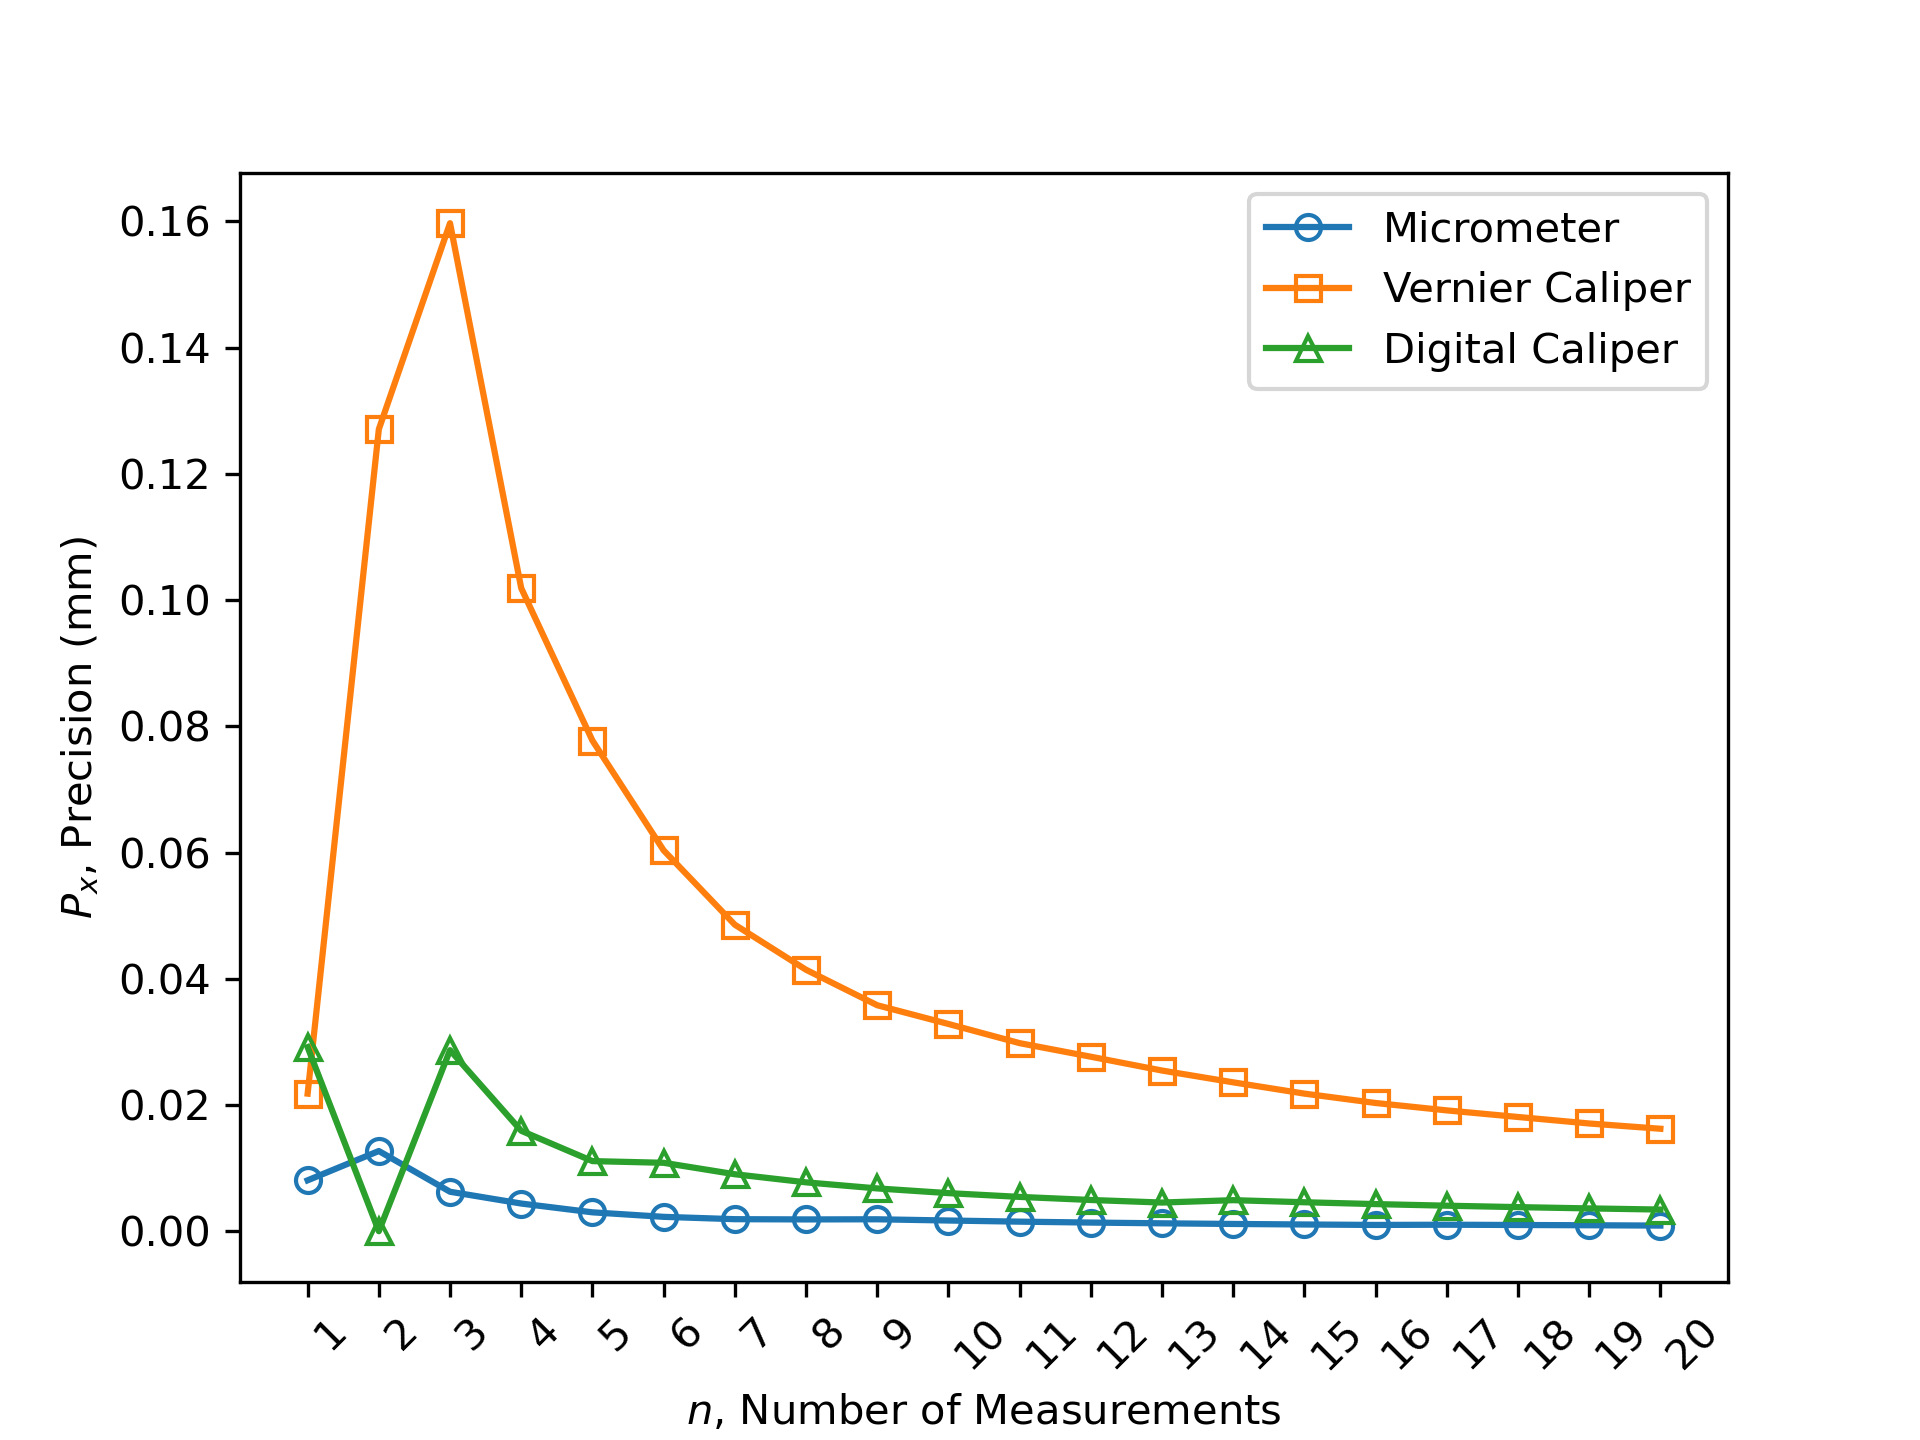
\includegraphics[width=0.8\linewidth]{Questions/Plots/Q3_Precision.png}
    \caption{Precision of various  measurement devices as measurement count increases} 
    \label{fig:precision-of-measurement-devices}
\end{figure}

\begin{figure}[h]
    \centering
    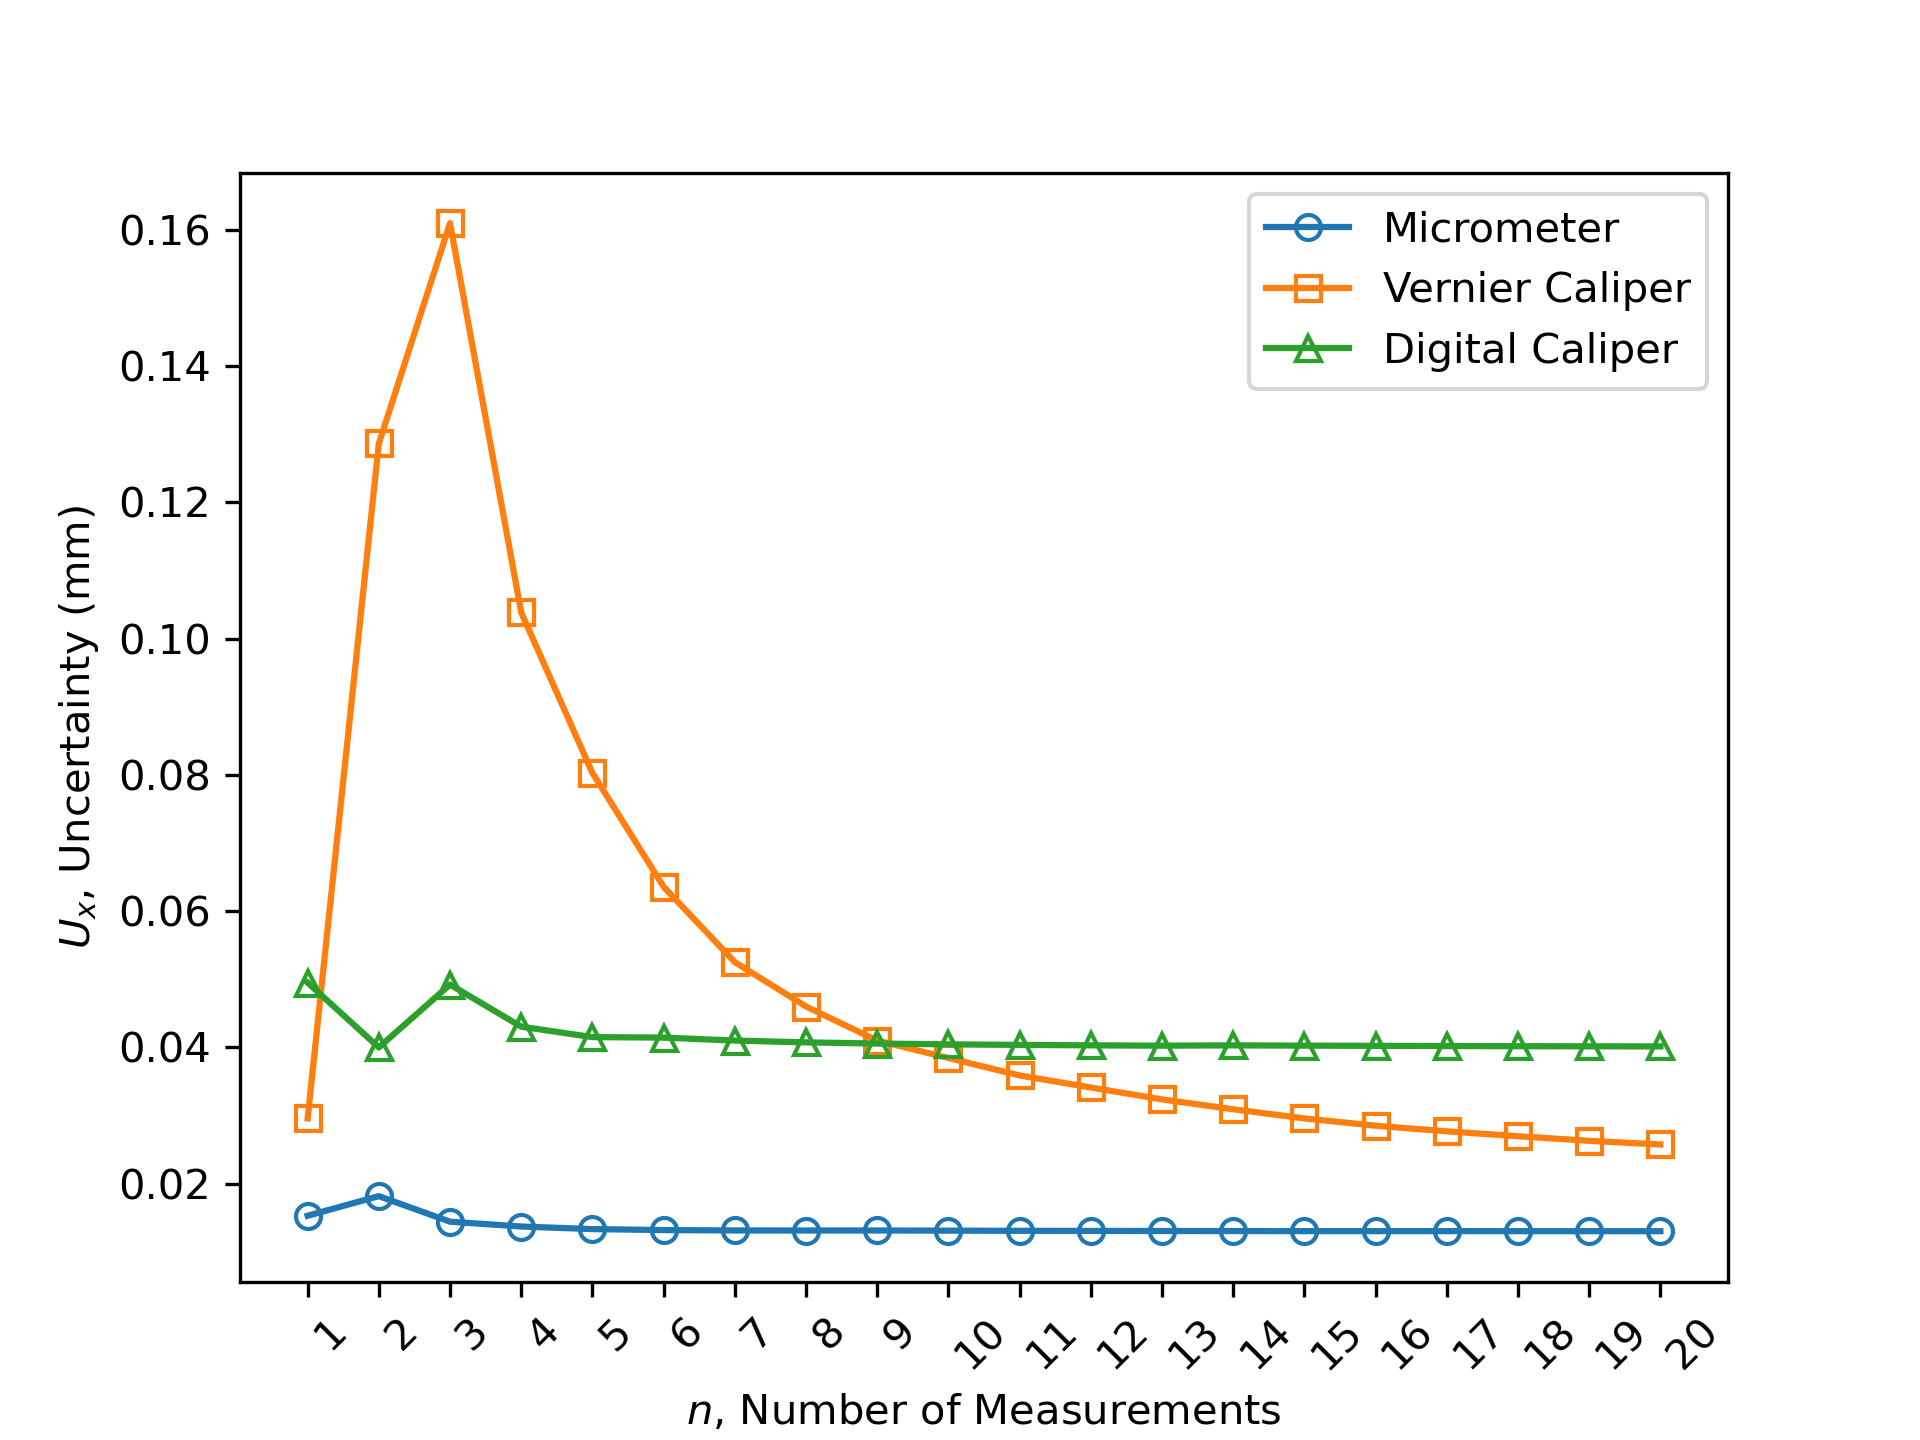
\includegraphics[width=0.8\linewidth]{Questions/Plots/Q3_Uncertainty.png}
    \caption{Uncertainty of various measurement devices as measurement count increases}
    \label{fig:uncertainty-of-measurement-devices}
\end{figure}

\FloatBarrier
\subsection{}
Since the formula for the precision is a function of one-sided t-distribution inverse as well as standard deviation, both of which decrease as the number of measurements increases, the precision will generally decrease as the number of measurements increases. The $\sum_{i=1}^{n} (x_i - \bar{x})^2$ term contributes a lot while n is small so standard deviation may not decrease for the first couple of terms. A crude guess is that the precision will decrease $\propto \frac{1}{n}$.\\

\noindent The formula for uncertainty is a function of precision and bias/accuracy. Accuracy is also reliant on the deviation of the measurements and will often reach a stable value after a certain number of measurements. If accuracy is approximately constant, the only contributing term would be the precision. Therefore, the uncertainty will probably decrease around $\propto \frac{1}{n}$ (not too familiar with the behaviour of inverse one-sided t-distribution).
 